\documentclass[border=5pt]{standalone}
% Shared by every figure. Colour marks the TYPE of a quantity, never decoration:
%   blue   (vec) equivariant: rotates with its fragment     -- solid arrows
%   orange (inv) invariant: unchanged by any rotation        -- dashed arrows
%   aqua   (att) attention / communication between elements
%   violet (out) what the network outputs
% Text is always ink; a coloured mark next to it carries the meaning.
\usepackage{amsmath,amssymb,bm}
\usepackage{tikz}
\usetikzlibrary{arrows.meta,positioning,fit,backgrounds,calc,shapes.geometric,
  shapes.misc,decorations.pathreplacing,decorations.pathmorphing,matrix,
  patterns,cd,shadows}
\definecolor{vec}{HTML}{2A78D6}
\definecolor{inv}{HTML}{EB6834}
\definecolor{att}{HTML}{1BAF7A}
\definecolor{out}{HTML}{4A3AA7}
\definecolor{ink}{HTML}{0B0B0B}
\definecolor{ink2}{HTML}{52514E}
\definecolor{ink3}{HTML}{8A877F}
\definecolor{neutral}{HTML}{F0EFEC}
\definecolor{rule}{HTML}{CFCCC4}
\definecolor{pieceA}{HTML}{E4E1DA}
\definecolor{pieceB}{HTML}{CDC9BF}
\definecolor{pieceC}{HTML}{B3AEA2}
\colorlet{vecfill}{vec!9}
\colorlet{invfill}{inv!10}
\colorlet{attfill}{att!11}
\colorlet{outfill}{out!9}
\tikzset{
  >={Stealth[length=2.3mm,width=1.7mm]},
  every picture/.style={line cap=round, line join=round},
  box/.style={draw=ink2, fill=neutral, rounded corners=2.5pt, align=center,
    font=\small, inner sep=4pt, minimum height=8mm, text=ink, line width=0.6pt, nohyph},
  vecbox/.style={box, draw=vec, fill=vecfill},
  invbox/.style={box, draw=inv, fill=invfill},
  attbox/.style={box, draw=att, fill=attfill},
  outbox/.style={box, draw=out, fill=outfill},
  plain/.style={box, draw=ink3, fill=white},
  arr/.style={->, draw=ink2, line width=0.7pt},
  vecarr/.style={->, draw=vec, line width=1.1pt},
  invarr/.style={->, draw=inv, line width=1.1pt, dash pattern=on 3.2pt off 1.8pt},
  attarr/.style={->, draw=att, line width=1.1pt, dash pattern=on 1.2pt off 1.4pt},
  outarr/.style={->, draw=out, line width=1.1pt},
  nohyph/.style={execute at begin node={\hyphenpenalty=10000\exhyphenpenalty=10000\relax}},
  lbl/.style={font=\footnotesize, text=ink2, align=center, nohyph},
  tlbl/.style={font=\footnotesize, text=ink, align=center, nohyph},
  group/.style={draw=ink3, dashed, rounded corners=5pt, inner sep=7pt},
  op/.style={circle, draw=ink2, fill=white, inner sep=0pt, minimum size=5.2mm,
    font=\small, line width=0.6pt},
  piece/.style={fill=#1, draw=none},
  intact/.style={draw=ink2, line width=0.6pt},
  fracture/.style={draw=ink, line width=1.5pt},
  token/.style={circle, fill=att, draw=white, line width=0.5pt, inner sep=0pt,
    minimum size=4.2pt},
  vtx/.style={circle, fill=ink, inner sep=0pt, minimum size=3pt},
  panel/.style={font=\small\bfseries, text=ink, anchor=north west},
}
% one piece of the cartoon, in its own centred frame: fill, intact edge, fracture edge
\newcommand{\drawpiece}[2]{% #1 = A|B|C, #2 = fill colour
  \fill[#2] \csname Piece#1\endcsname;
  \draw[intact] \csname Intact#1\endcsname;
  \draw[fracture] \csname Crack#1\endcsname;}
% a legend entry: a short line in a given style, then its text
\newcommand{\legendline}[3]{% #1 position, #2 style, #3 text
  \draw[#2] (#1) -- ++(0.7,0) node[right, tlbl, text=ink] {#3};}

\begin{document}
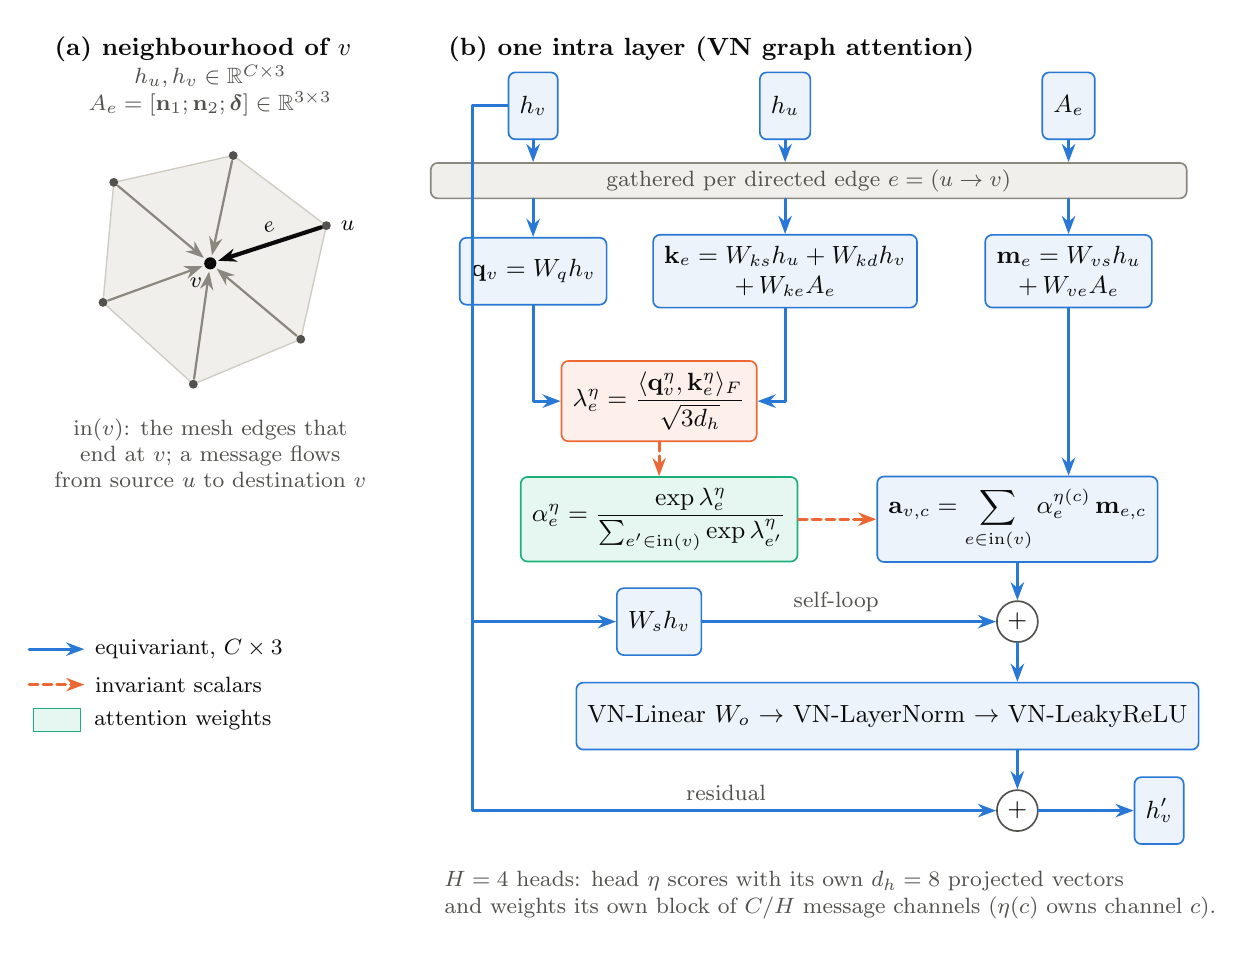
\begin{tikzpicture}
  \tikzset{
    fb/.style={font=\small, minimum height=8.5mm},
    note/.style={lbl, anchor=west, align=left},
  }
  % =================== (a) the neighbourhood of v ===================
  \node[panel] at (-5.35,1.0) {(a) neighbourhood of $v$};
  \begin{scope}[shift={(-3.25,-2.0)}]
    \coordinate (v) at (0,0);
    \foreach \k/\a/\r in {1/18/1.55,2/78/1.4,3/140/1.6,4/200/1.45,5/262/1.55,6/320/1.5}{
      \coordinate (u\k) at (\a:\r);}
    \foreach \a/\b in {1/2,2/3,3/4,4/5,5/6,6/1}{
      \fill[neutral] (v) -- (u\a) -- (u\b) -- cycle;
      \draw[rule, line width=0.5pt] (u\a) -- (u\b);}
    \foreach \k in {2,...,6}{
      \draw[->, ink3, line width=0.8pt, shorten >=3pt, shorten <=2pt] (u\k) -- (v);}
    \draw[->, ink, line width=1.5pt, shorten >=3pt, shorten <=2pt] (u1) -- (v)
      node[pos=0.45, above, tlbl, sloped] {$e$};
    \foreach \k in {1,...,6}{\fill[ink2] (u\k) circle (1.6pt);}
    \fill[ink] (v) circle (2.2pt);
    \node[tlbl, anchor=north east] at ($(v)+(0.02,-0.06)$) {$v$};
    \node[tlbl, anchor=west] at ($(u1)+(0.06,0)$) {$u$};
    \node[lbl, anchor=north, align=center] at (0,-1.85)
      {$\mathrm{in}(v)$: the mesh edges that\\ end at $v$; a message flows\\ from source $u$ to destination $v$};
    \node[lbl, anchor=south, align=center] at (0,1.75)
      {$h_u,h_v\in\mathbb R^{C\times 3}$\\ $A_e=[\mathbf n_1;\mathbf n_2;\boldsymbol\delta]\in\mathbb R^{3\times3}$};
  \end{scope}

  % =================== (b) the layer ===================
  \node[panel] at (-0.35,1.0) {(b) one intra layer (VN graph attention)};
  \node[vecbox, fb] (hv) at (0.85,0) {$h_v$};
  \node[vecbox, fb] (hu) at (4.05,0) {$h_u$};
  \node[vecbox, fb] (ae) at (7.65,0) {$A_e$};
  \node[box, draw=ink3, fill=neutral, minimum height=4.5mm, inner sep=1.5pt, font=\footnotesize, text=ink2,
        minimum width=9.6cm] (bus) at (4.35,-0.95) {gathered per directed edge $e=(u\to v)$};
  \foreach \n in {hv,hu,ae}{\draw[vecarr] (\n) -- (\n |- bus.north);}
  \node[vecbox, fb] (q) at (0.85,-2.1) {$\mathbf q_v=W_q h_v$};
  \node[vecbox, fb, align=center] (k) at (4.05,-2.1) {$\mathbf k_e=W_{ks}h_u+W_{kd}h_v$\\ $+\,W_{ke}A_e$};
  \node[vecbox, fb, align=center] (m) at (7.65,-2.1) {$\mathbf m_e=W_{vs}h_u$\\ $+\,W_{ve}A_e$};
  \foreach \n in {q,k,m}{\draw[vecarr] (\n |- bus.south) -- (\n);}
  % score and softmax
  \node[invbox, fb] (s) at (2.45,-3.75)
    {$\lambda_e^{\eta}=\dfrac{\langle\mathbf q_v^{\eta},\mathbf k_e^{\eta}\rangle_F}{\sqrt{3d_h}}$};
  \draw[vecarr] (q.south) |- (s.west);
  \draw[vecarr] (k.south) |- (s.east);
  \node[attbox, fb] (a) at (2.45,-5.25)
    {$\alpha_e^{\eta}=\dfrac{\exp\lambda_e^{\eta}}{\sum_{e'\in\mathrm{in}(v)}\exp\lambda_{e'}^{\eta}}$};
  \draw[invarr] (s) -- (a);
  % aggregation
  \node[vecbox, fb] (g) at (7.0,-5.25) {$\displaystyle\mathbf a_{v,c}=\sum_{e\in\mathrm{in}(v)}\alpha_e^{\eta(c)}\,\mathbf m_{e,c}$};
  \draw[invarr] (a) -- (g);
  \draw[vecarr] (m.south) -- (m.south |- g.north);
  % self-loop, output transform, residual
  \node[op] (plus) at (7.0,-6.55) {$+$};
  \draw[vecarr] (g) -- (plus);
  \node[vecbox, fb] (self) at (2.45,-6.55) {$W_s h_v$};
  \draw[vecarr] (self) -- (plus);
  \draw[vecarr] (hv.west) -- ++(-0.45,0) |- (self.west);
  \node[vecbox, fb] (out) at (5.35,-7.75) {VN-Linear $W_o$ $\to$ VN-LayerNorm $\to$ VN-LeakyReLU};
  \draw[vecarr] (plus) -- (plus |- out.north);
  \node[op] (res) at (7.0,-8.95) {$+$};
  \draw[vecarr] (plus |- out.south) -- (res);
  \draw[vecarr] (hv.west) -- ++(-0.45,0) |- (res.west);
  \node[vecbox, fb] (new) at (8.8,-8.95) {$h_v'$};
  \draw[vecarr] (res) -- (new);
  \node[lbl, anchor=south] at (3.3,-8.95) {residual};
  \node[lbl, anchor=south] at (4.7,-6.55) {self-loop};
  % heads note and legend
  \node[note, anchor=north west] at (-0.4,-9.6) {$H=4$ heads: head $\eta$ scores with its own $d_h=8$ projected vectors\\
    and weights its own block of $C/H$ message channels ($\eta(c)$ owns channel $c$).};
  \begin{scope}[shift={(-5.55,-6.9)}]
    \draw[vecarr] (0,0) -- (0.7,0) node[right, tlbl] {equivariant, $C\times3$};
    \draw[invarr] (0,-0.45) -- (0.7,-0.45) node[right, tlbl] {invariant scalars};
    \fill[attfill, draw=att] (0.05,-1.05) rectangle (0.65,-0.75);
    \node[right, tlbl] at (0.7,-0.9) {attention weights};
  \end{scope}
\end{tikzpicture}
\end{document}
